\section{Solution exacte de Maxwell sur une sphère: la série de Mie}\label{sec_serie_mie}
%TODO

\TODO{refaire cette partie et expliquer la somme finale sur les champs}

Maintenant que nous connaissons l'ensemble des solutions de Maxwell ainsi que la manière s'approcher la condition d'impédance, nous allons expliciter les coefficients $(a_n,b_n)$  afin d'assurer le condition d'impédance de surface.

% Le but est de déterminer les coefficients qui permettent de décomposer les champs sur les harmoniques sphériques pour aboutir aux séries de Mie, et de déterminer les coefficients de Mie $(a_n,b_n)$

\subsection{Rappel}
Soit $\O = B_{\R^3}(0,R)$, $M_{m,n}, N_{m,n}$ les harmoniques sphériques (cf \cite{marceaux_high-order_2000} et section \ref{sec_sol_maxwell})

% Dans la base sphérique :
% \[
%   M_{m,n}=
%   \begin{pmatrix}
%     0\\
%     ime^{im\phi}\frac{\mathbb{P}^m_n(\cos\theta)}{\sin\theta}\\
%     -e^{im\phi}\dd{\theta}{\mathbb{P}^m_n(\cos\theta)}\\
%   \end{pmatrix}
%   \qquad
%   N_{m,n}=
%   \begin{pmatrix}
%     n(n+1)e^{im\phi}\frac{\mathbb{P}^m_n(\cos\theta)}{k_0r}\int_0^x( Id\, dt)/x\\
%     \frac{e^{im\phi}}{k_0r}\dd{\theta}{\mathbb{P}^m_n(\cos\theta)}Id\\
%     im\frac{e^{im\phi}}{k_0r\sin\theta}\mathbb{P}^m_n(\cos\theta)Id
%   \end{pmatrix}
% \]

On pose
\begin{align*}
  \gls{mat-conj} &=conj(z)\\
  \gls{mat-gmn} &=\frac{4\pi}{2n+1}n(n+1)\frac{(n+m)!}{(n-m)!}\\
  \gls{mat-tild} &= \dr{x}{(xu(x))}
\end{align*}

D'après les résultats énoncés en \ref{sec_helmholtz_scal}, on a
\[
  j_n(k_0r)M_{m,n} = j_n(k_0r)
  \begin{pmatrix}
    0\\
    ime^{im\phi}\frac{\mathbb{P}^m_n(\cos\theta)}{\sin\theta}\\
    -e^{im\phi}\dd{\theta}{\mathbb{P}^m_n(\cos\theta)}\\
  \end{pmatrix}
\]
et 
\[
  \tilde{j_n}(k_0r)N_{m,n}=
    \begin{pmatrix}
    n(n+1)e^{im\phi}\frac{\mathbb{P}^m_n(\cos\theta)}{k_0r}j_n(k_0r)\\
    \frac{e^{im\phi}}{k_0r}\dd{\theta}{\mathbb{P}^m_n(\cos\theta)}\tilde j_n(k_0r)\\
    im\frac{e^{im\phi}}{k_0r\sin\theta}\mathbb{P}^m_n(\cos\theta)\tilde j_n(k_0r)
  \end{pmatrix}
\]

On a donc les expressions suivantes pour les champs $(\E,\H)$ solution de Maxwell, sans condition de rayonnement:
$\forall m,n \Z\pvect\N$




On rappelle les relations vectorielles liant $M$ et $N$
\begin{align*}
  &\v e_r \pvect N_{1,n} = -\frac{1}{k_0r}M_{1,n} \\
  &\v e_r \pvect M_{1,n} = k_0r N_{1,n}^t
\end{align*}

\subsection{Expression des champs solutions de Maxwell}
Soient $(a_n,b_n)_n$ des suites complexes, $f_n = \frac{i^{n+1}(2n+1)}{2n(n+1)}$.

D’après \cite{morse_methods_1953}, les solutions $(\E,\H)$ (avec $\H \equiv \H /\eta_0 $) sont :
\begin{align*}
  \E^i &= -\sum_{n=1}^\infty f_n \left( j_nM_{1,n} + \tilde j_n N_{1,n} \right) + n(n+1)\left(j_n M_{-1,n} - \tilde j_nN_{-1,n} \right)\\
  \H^i &= -i\sum_{n=1}^\infty f_n \left( j_nM_{1,n} + \tilde j_nN_{1,n} \right) - n(n+1)\left(j_n M_{-1,n} - \tilde j_n N_{-1,n} \right)\\
  \E^d &= -\sum_{n=1}^\infty f_n \left( a_n h_nM_{1,n} + b_n\tilde h_nN_{1,n} \right) + n(n+1)\left(a_nh_nM_{-1,n} - b_n\tilde h_nN_{-1,n} \right)\\
  \H^d &= -i\sum_{n=1}^\infty f_n \left( b_nh_nM_{1,n} + a_n\tilde h_nN_{1,n} \right) - n(n+1)\left(b_nh_nM_{-1,n} - a_n\tilde h_nN_{-1,n} \right)\\
\end{align*}
Et les champs totaux solution de Maxwell sont : 
\begin{align}
  \E = \E^i + \E^d\label{eq_solEmie}\\
  \H = \H^i + \H^d\label{eq_solHmie}
\end{align}

On rappelle les relation d'orthogonalités énoncées dans \cite{marceaux_high-order_2000}, avec $\delta$ le symbole de Kronecker :
\[
  \begin{matrix}
    \ds\int_S \div N_{m,n}^t \div N_{p,q}^{t,*} &=& \frac{n(n+1)}{k_0^2 R^2} \gamma_{m,n} \delta_{m,n} \delta_{p,q}\\
    \ds\int_S N_{m,n}^t \cdot N_{p,q}^{t,*} &=& \frac{1}{k_0^2}\gamma_{m,n}\delta_{m,n} \delta_{p,q}\\
    \ds\int_S \left(\v e_r \cdot \rot M_{m,n}\right)\left( e_r \cdot \rot  M_{p,q}^{*}\right) &=& n(n+1) \gamma_{m,n} \delta_{m,n} \delta_{p,q}\\
    \ds\int_S M_{m,n} \cdot M_{p,q}^{*} &=& R^2 \gamma_{m,n} \delta_{m,n} \delta_{p,q}\\
    \ds\int_S M_{m,n} \cdot N_{p,q}^{t,*} &=& 0
  \end{matrix}
\]
Et les relations différentielles suivantes:
\begin{align*}
  \div M_{m,n} &=0 \\
  \v e_r \cdot \rot N_{m,n} &= 0
\end{align*}

\subsection{Calcul des coefficients de la série de Mie.}
\textbf{Rappel : Sauf mention contraire, les $h_n,j_n$ sont calculées au point $k_0R$. On omet donc cette dépendance dans l'écriture.}\\
Le but est d'expliciter la \gls{acr-cioe} pour trouver des $a_n, b_n$ la satisfaisant.
Soit $k_0 = w\sqrt{\eps_0\mu_0}$
\begin{equation}
  \label{eq_CIOE} \left(1+\frac{b}{k_0^2}L\right)\E_t\ = \left(a_0 + \frac{a_1}{k_0^2}L\right)\J
\end{equation}
L est l'opérateur tel que 
\[
  \int_{S} L(u)\cdot v = - \int_{S} {\div u}_t {\div v}_t - \int_{S}\left(\n \cdot \rot u\right)\left( \n \cdot \rot v\right)
\]
\subsubsection{Obtention des $a_n$}
On intègre cette relation après un produit scalaire avec $M_{1,n}^{*}$ et l'on va expliciter chaque terme:
\begin{align*}
  &\int_S \E_t\cdot M_{1,n}^{*} = - f_n R^2 \gamma_{1,n}[a_n h_n + j_n]\\
  &\int_S L(\E_t)\cdot M_{1,n}^{*} =  f_n n(n+1)\gamma_{1,n}[a_n h_n + j_n]\\
  &\int_S \J \cdot M_{1,n}^{*} =  i f_n \frac{R}{k_0} \gamma_{1,n}[a_n \tilde h_n + \tilde j_n]\\
  &\int_S L(\J) \cdot M_{1,n}^{*} =  - i f_n n(n+1) \gamma_{1,n}\frac{1}{k_0 R}[a_n \tilde h_n + \tilde j_n]\\
\end{align*}
En combinant l'ensemble de ces termes, on obtient les $a_n$:

Soit $ \alpha_n =-i\frac{a_0R^2k^2 - a_1 n (n+1)}{k^2R^2 - bn(n+1)}$, alors
\begin{equation}
  \label{eq_an_mie} a_n = -\frac{\tilde{j_n}\frac{1}{k_0R}\alpha_n +j_n}{\tilde{h_n}\frac{1}{k_0R}\alpha_n + h_n}
\end{equation}

\subsubsection{Obtention des $b_n$}
On intègre cette relation après un produit scalaire avec $N_{1,n}^{t,*}$ et l'on va expliciter chaque terme:
\begin{align*}
  &\int_S \E_t\cdot N_{1,n}^{t,*} = - f_n \frac{1}{k_0^2} \gamma_{1,n}[b_n\tilde{h_n} + \tilde{j_n} ]\\
  &\int_S L(\E_t)\cdot N_{1,n}^{t,*} =  f_n \frac{n(n+1)}{k_0^2R^2}\gamma_{1,n}[b_n\tilde{h_n} + \tilde{j_n}]\\
  &\int_S \J \cdot N_{1,n}^{t,*} = - i f_n \frac{R}{k_0}\gamma_{1,n}[b_n {h_n} + {j_n}]\\
  &\int_S L(\J) \cdot N_{1,n}^{t,*} =  i f_n \frac{n(n+1)}{k_0 R} \gamma_{1,n}[b_n {h_n} + {j_n}]\\
\end{align*}
En combinant l'ensemble de ces termes, on obtient les $b_n$ :

%FIXME : corriger équation ci dessous
\begin{equation}
  \label{eq_bn_mie} b_n = -\frac{\tilde{j_n}- \frac{R}{k_0}\alpha_n j_n}{\tilde{h_n}-\frac{R}{k_0}\alpha_nh_n}
\end{equation}
\subsection{Lien entre des CSU et Q}
\textbf{Rappel:} $\ds Q=\Re{\int_{\d\Omega}\J\cdot(\conj{\E_t})ds}$

En utilisant les relations d'orthogonalités et $\gamma_{1,n} = n(n+1)\gamma_{-1,n}$, on trouve
\[
  Q = \sum_ {n=0}^{\infty}2\gamma_{1,n}\frac{|f_n|^2R}{k_0}\Im{
  \left[
    (a_n h_n + j_n)(a_n^* \tilde h_n^* + \tilde j_n^*) 
    %- (b_n \tilde h_n + \tilde j_n)(b_n^*  h_n^* + j_n^*)
  \right]}
\]

\iffalse
\subsection{Notes, remarques}
Étant donnée la CI dans \cite{marceaux_high-order_2000} en $\n \pvect \E = Z \H_t$ et avec le fait qu'il intègre sur l'intérieur donc avec $M^i, N^i$, mes expressions des $a_n,b_n$ sont différentes, mais dans le même ordre d'idée : 
\[
a_n \mapsto b_n, \alpha_n \mapsto - i \eta_0/\eta k \alpha_n^{-1}
\]
\[
b_n \mapsto a_n, \beta_n \mapsto - i \eta_0/\eta k \beta_n^{-1}
\]
\fi


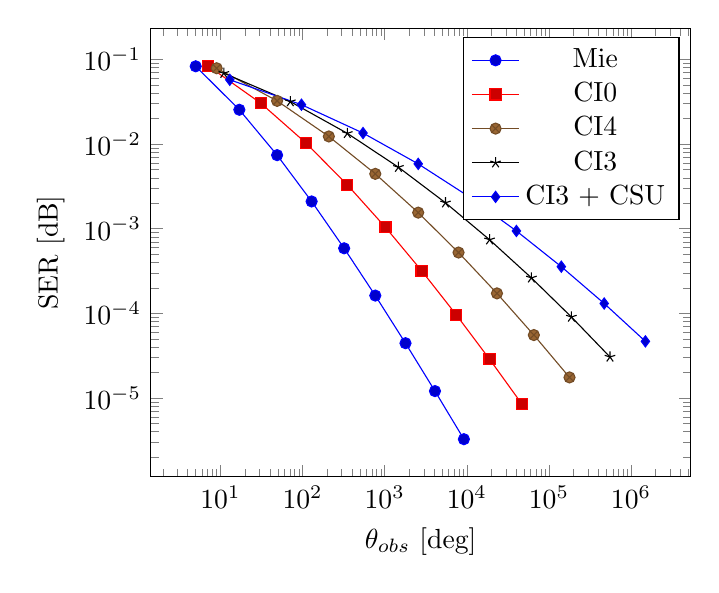
\begin{tikzpicture}
\begin{loglogaxis}[
    xlabel={$\theta_{obs}$ [deg]},
    ylabel={SER [dB]}
]
\addplot coordinates {
    (5,8.312e-02)    (17,2.547e-02)   (49,7.407e-03)
    (129,2.102e-03)  (321,5.874e-04)  (769,1.623e-04)
    (1793,4.442e-05) (4097,1.207e-05) (9217,3.261e-06)
};

\addplot coordinates{
    (7,8.472e-02)    (31,3.044e-02)    (111,1.022e-02)
    (351,3.303e-03)  (1023,1.039e-03)  (2815,3.196e-04)
    (7423,9.658e-05) (18943,2.873e-05) (47103,8.437e-06)
};

\addplot coordinates{
    (9,7.881e-02)     (49,3.243e-02)    (209,1.232e-02)
    (769,4.454e-03)   (2561,1.551e-03)  (7937,5.236e-04)
    (23297,1.723e-04) (65537,5.545e-05) (178177,1.751e-05)
};

\addplot coordinates{
    (11,6.887e-02)    (71,3.177e-02)     (351,1.341e-02)
    (1471,5.334e-03)  (5503,2.027e-03)   (18943,7.415e-04)
    (61183,2.628e-04) (187903,9.063e-05) (553983,3.053e-05)
};

\addplot coordinates{
    (13,5.755e-02)     (97,2.925e-02)     (545,1.351e-02)
    (2561,5.842e-03)   (10625,2.397e-03)  (40193,9.414e-04)
    (141569,3.564e-04) (471041,1.308e-04) (1496065,4.670e-05)
};
\legend{Mie,CI0,CI4,CI3,CI3 + CSU}
\end{loglogaxis}
\end{tikzpicture}